%% System Design
%%=========================================

\chapter{System Design}
\label{ch:system_design}
The main objective of this thesis is to answer the research questions by creating a system, as established in by our choice of research strategy in Chapter \ref{ch:methodology} and method in Chapter \ref{ch:problem}. In this chapter, we present the design of the system we made. We present the general design in Section \ref{sec:general_design}, while Sections \ref{sec:preprocessor} and \ref{sec:transformator} presents the most essential components, namely the {\tt Preprocessor} and the {\tt Transformator}.

%%=========================================

\section{General Design}
\label{sec:general_design}
Our models use supervised learning, a task which revolves around two phases: training and testing. We designed our system specifically with this in mind.

The system consists of several separate modules, each responsible for its individual task. The two first modules are the {\tt Trainer} and the {\tt Tester}. These modules are responsible for starting whatever other modules are required to run before the actual training or testing can take place, as well as invoking the action on the correct model. The {\tt Preprocessor} is responsible for creating the datasets we use in both the training and testing phase. The {\tt Transformator} module ``transform'' the input and label data stored from the {\tt Preprocessor} into a format that the models expect. Finally, the system calls the {\tt Predictor} which loads the correct model and either starts training or testing it.

\begin{figure}[ht]
    \centering
    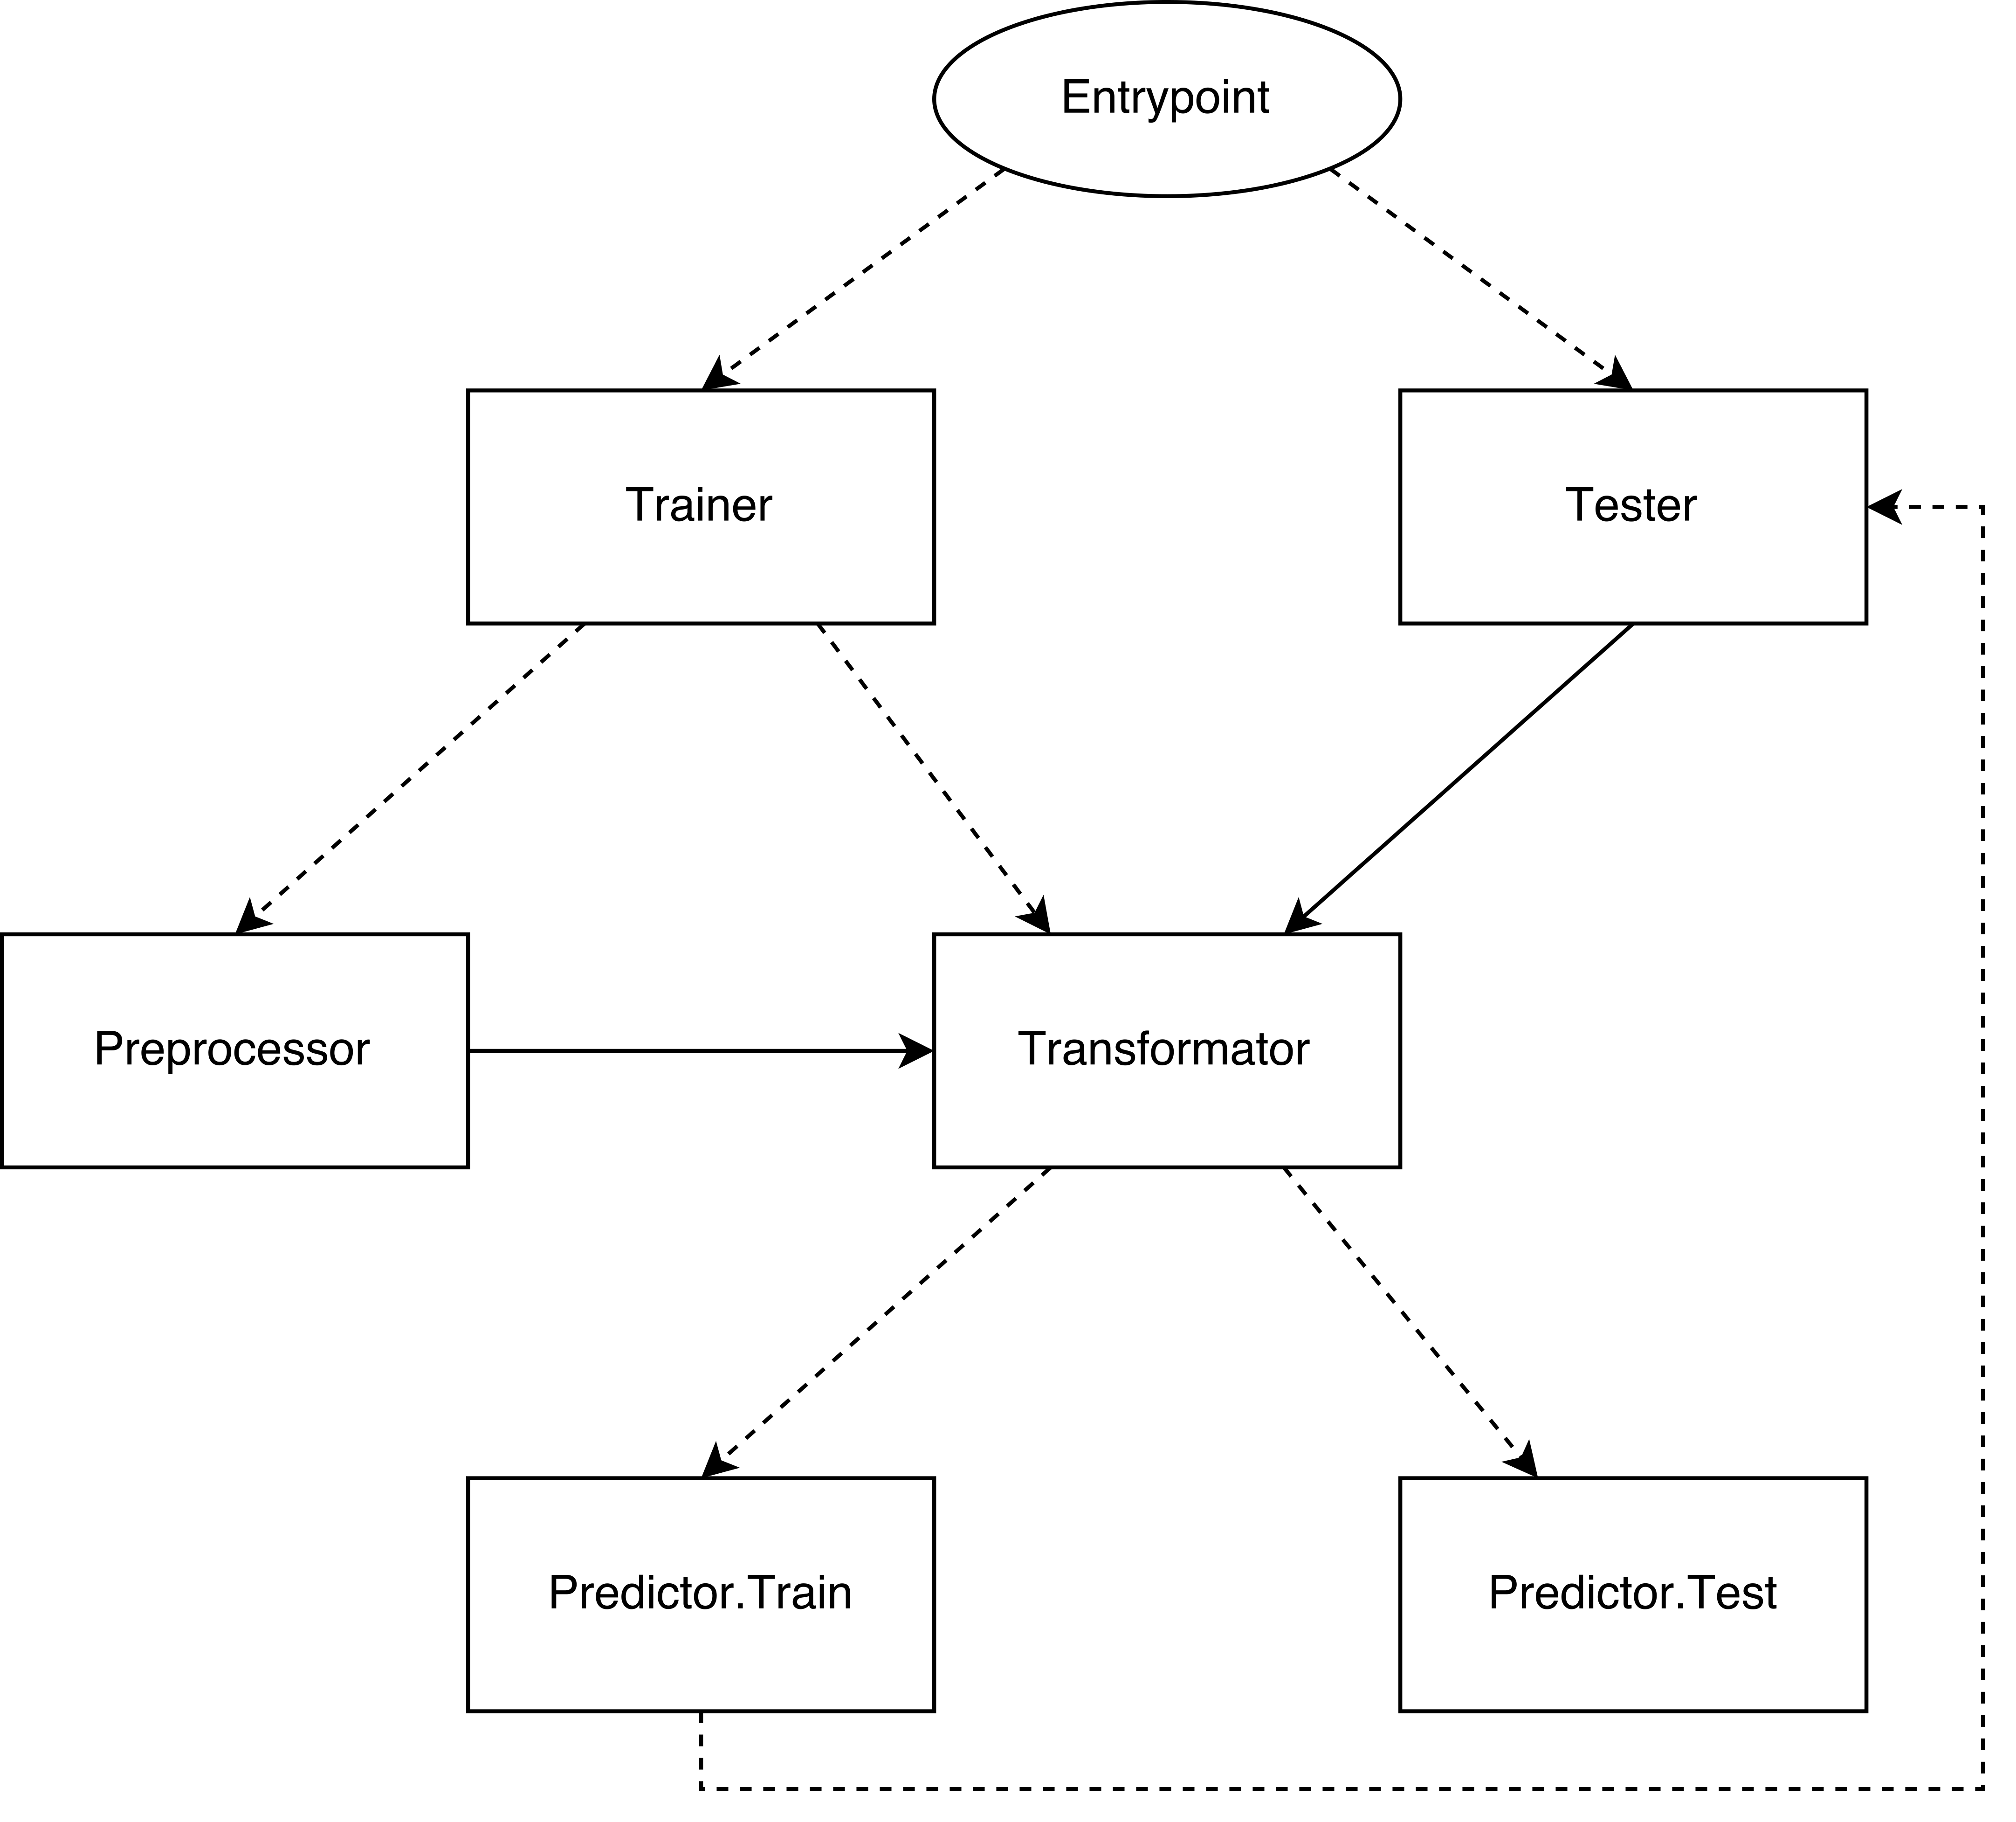
\includegraphics[width=0.7\textwidth]{fig/system_design/system_design.png}
    \caption{Simplified module interaction overview}
    \label{fig:system-design}
\end{figure}

Figure \ref{fig:system-design} presents a simplified overview of the system design, and how the modules fit together. A solid line indicates a direct route from one module to another, and a dashed line indicates that the module can take several routes. For example, the {\tt Trainer} module can either call {\tt Preprocessor} to create a new dataset, or it may call the {\tt Transformator} directly if it is asked to reuse an existing dataset.

%%=========================================

\section{Preprocessor}
\label{sec:preprocessor}
As there were no existing datasets suitable for our particular problem, we decided to create these ourselves. Creation of these datasets was done by implementing a configurable pipeline system that involved a process in several steps:

\begin{enumerate}
    \item Build a complete dictionary of words, make sure they only include allowed characters.
    \item Select random words from the list and construct training, validation, and test sets. Make sure no words exceeded the maximum word length configuration. Remove duplicated words both across lists and within the same list.
    \item Write the text from the lists on individual (empty) canvases, with the specified font type and font size.
    \item Find the boundaries of the characters and crop the text to remove the excessive space on the canvas.
    \item Apply the masks and extract the signature values.
    \item Save the final output.
\end{enumerate}

\begin{figure}[H]
    \centering
    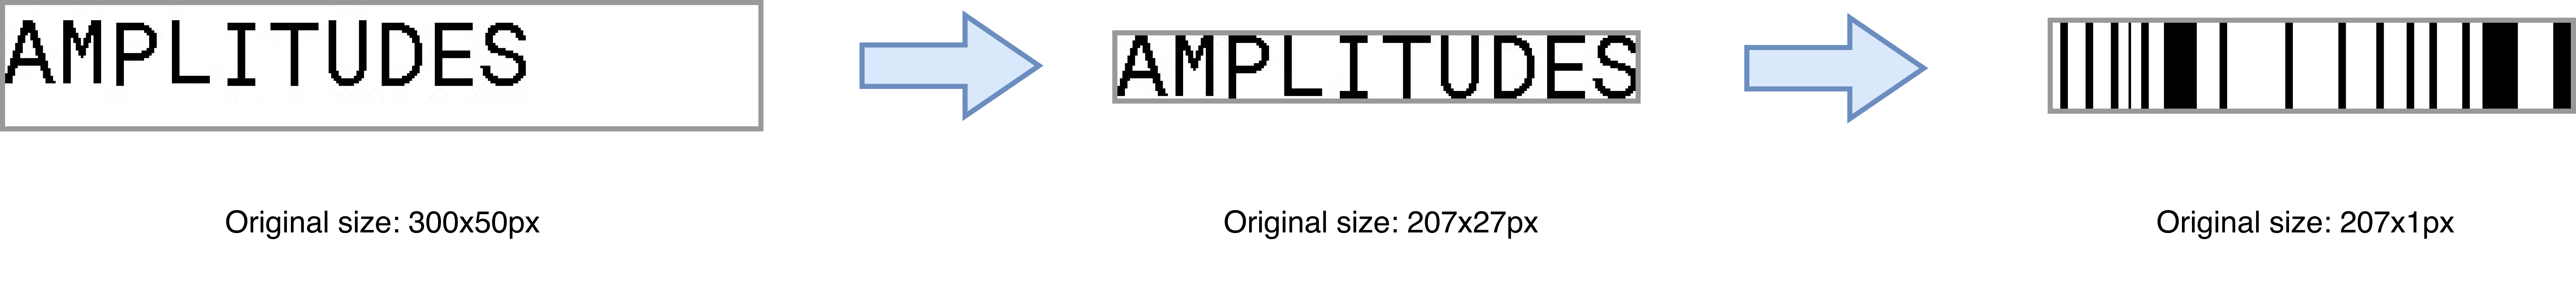
\includegraphics[width=1\textwidth]{fig/development_process/pipeline.png}
    \caption{Illustration of the pipeline process from canvas to signature}
    \label{fig:development-pipeline}
\end{figure}

Figure \ref{fig:development-pipeline} illustrates the steps done when writing out, cropping, and applying our signature to a word. First, we write out the word on a big, white canvas. This canvas has a predefined size, as we are unable to predict the actual size of the text before it is written out. The canvas is then cropped based on the boundaries calculated from the individual characters. Finally, we apply the masks to the cropped image and extract the pixels in the signature. In Figure \ref{fig:development-pipeline}, the rightmost subfigure illustrates the extracted signature from the middle subfigure, which has a height of one pixel and is masked fourteen pixels from the bottom. The signature was expanded vertically for increased visibility. The final signature sequence is extracted by iterating over the pixels in the image and is stored for later. In the illustrated example, the word ``AMPLITUDES'' results in a signature sequence that is 207 pixels long. This signature is stored as a binary vector with the same length.

\subsection{Multifont and Casing}
Special functionality was implemented in the pipeline process to create datasets with multiple fonts. The pipeline chooses one of \(N\) fonts, with an equal probability distribution (\(\frac{1}{N}\)) for each font.

Another method was implemented to change the casing of the words picked from the datasets. If the system were configured to include both upper-cased and lower-cased letters, the system will capitalize all the letters with probability 0.5.

%%=========================================

\section{Transformator}
\label{sec:transformator}
The {\tt Transformator} module was created to transform the sequences of binary data from the {\tt Preprocessor} into a format that the models expected. During development, especially in the early stages, the formats the models expected their inputs and output in varied. It, therefore, made sense to split the {\tt Preprocessor} and the {\tt Transformator} into separate modules which are executed in sequence. This allowed us to reuse the same dataset on multiple models that had different input and output format expectations.

The {\tt Transformator} is given a sequence of ``handlers'', depending on which model is to be loaded in the {\tt Predictor}. These handlers are executed in sequence, and each handler does a modification to either the input or the output format, and the data is propagated to the next handler. This way, the handlers could easily be reordered or swapped if a model expects another format. Typical tasks include padding the input to a given width, re-scaling the input to unsigned integers, or turning the output into a one-hot matrix.

\begin{figure}[ht]
    \centering
    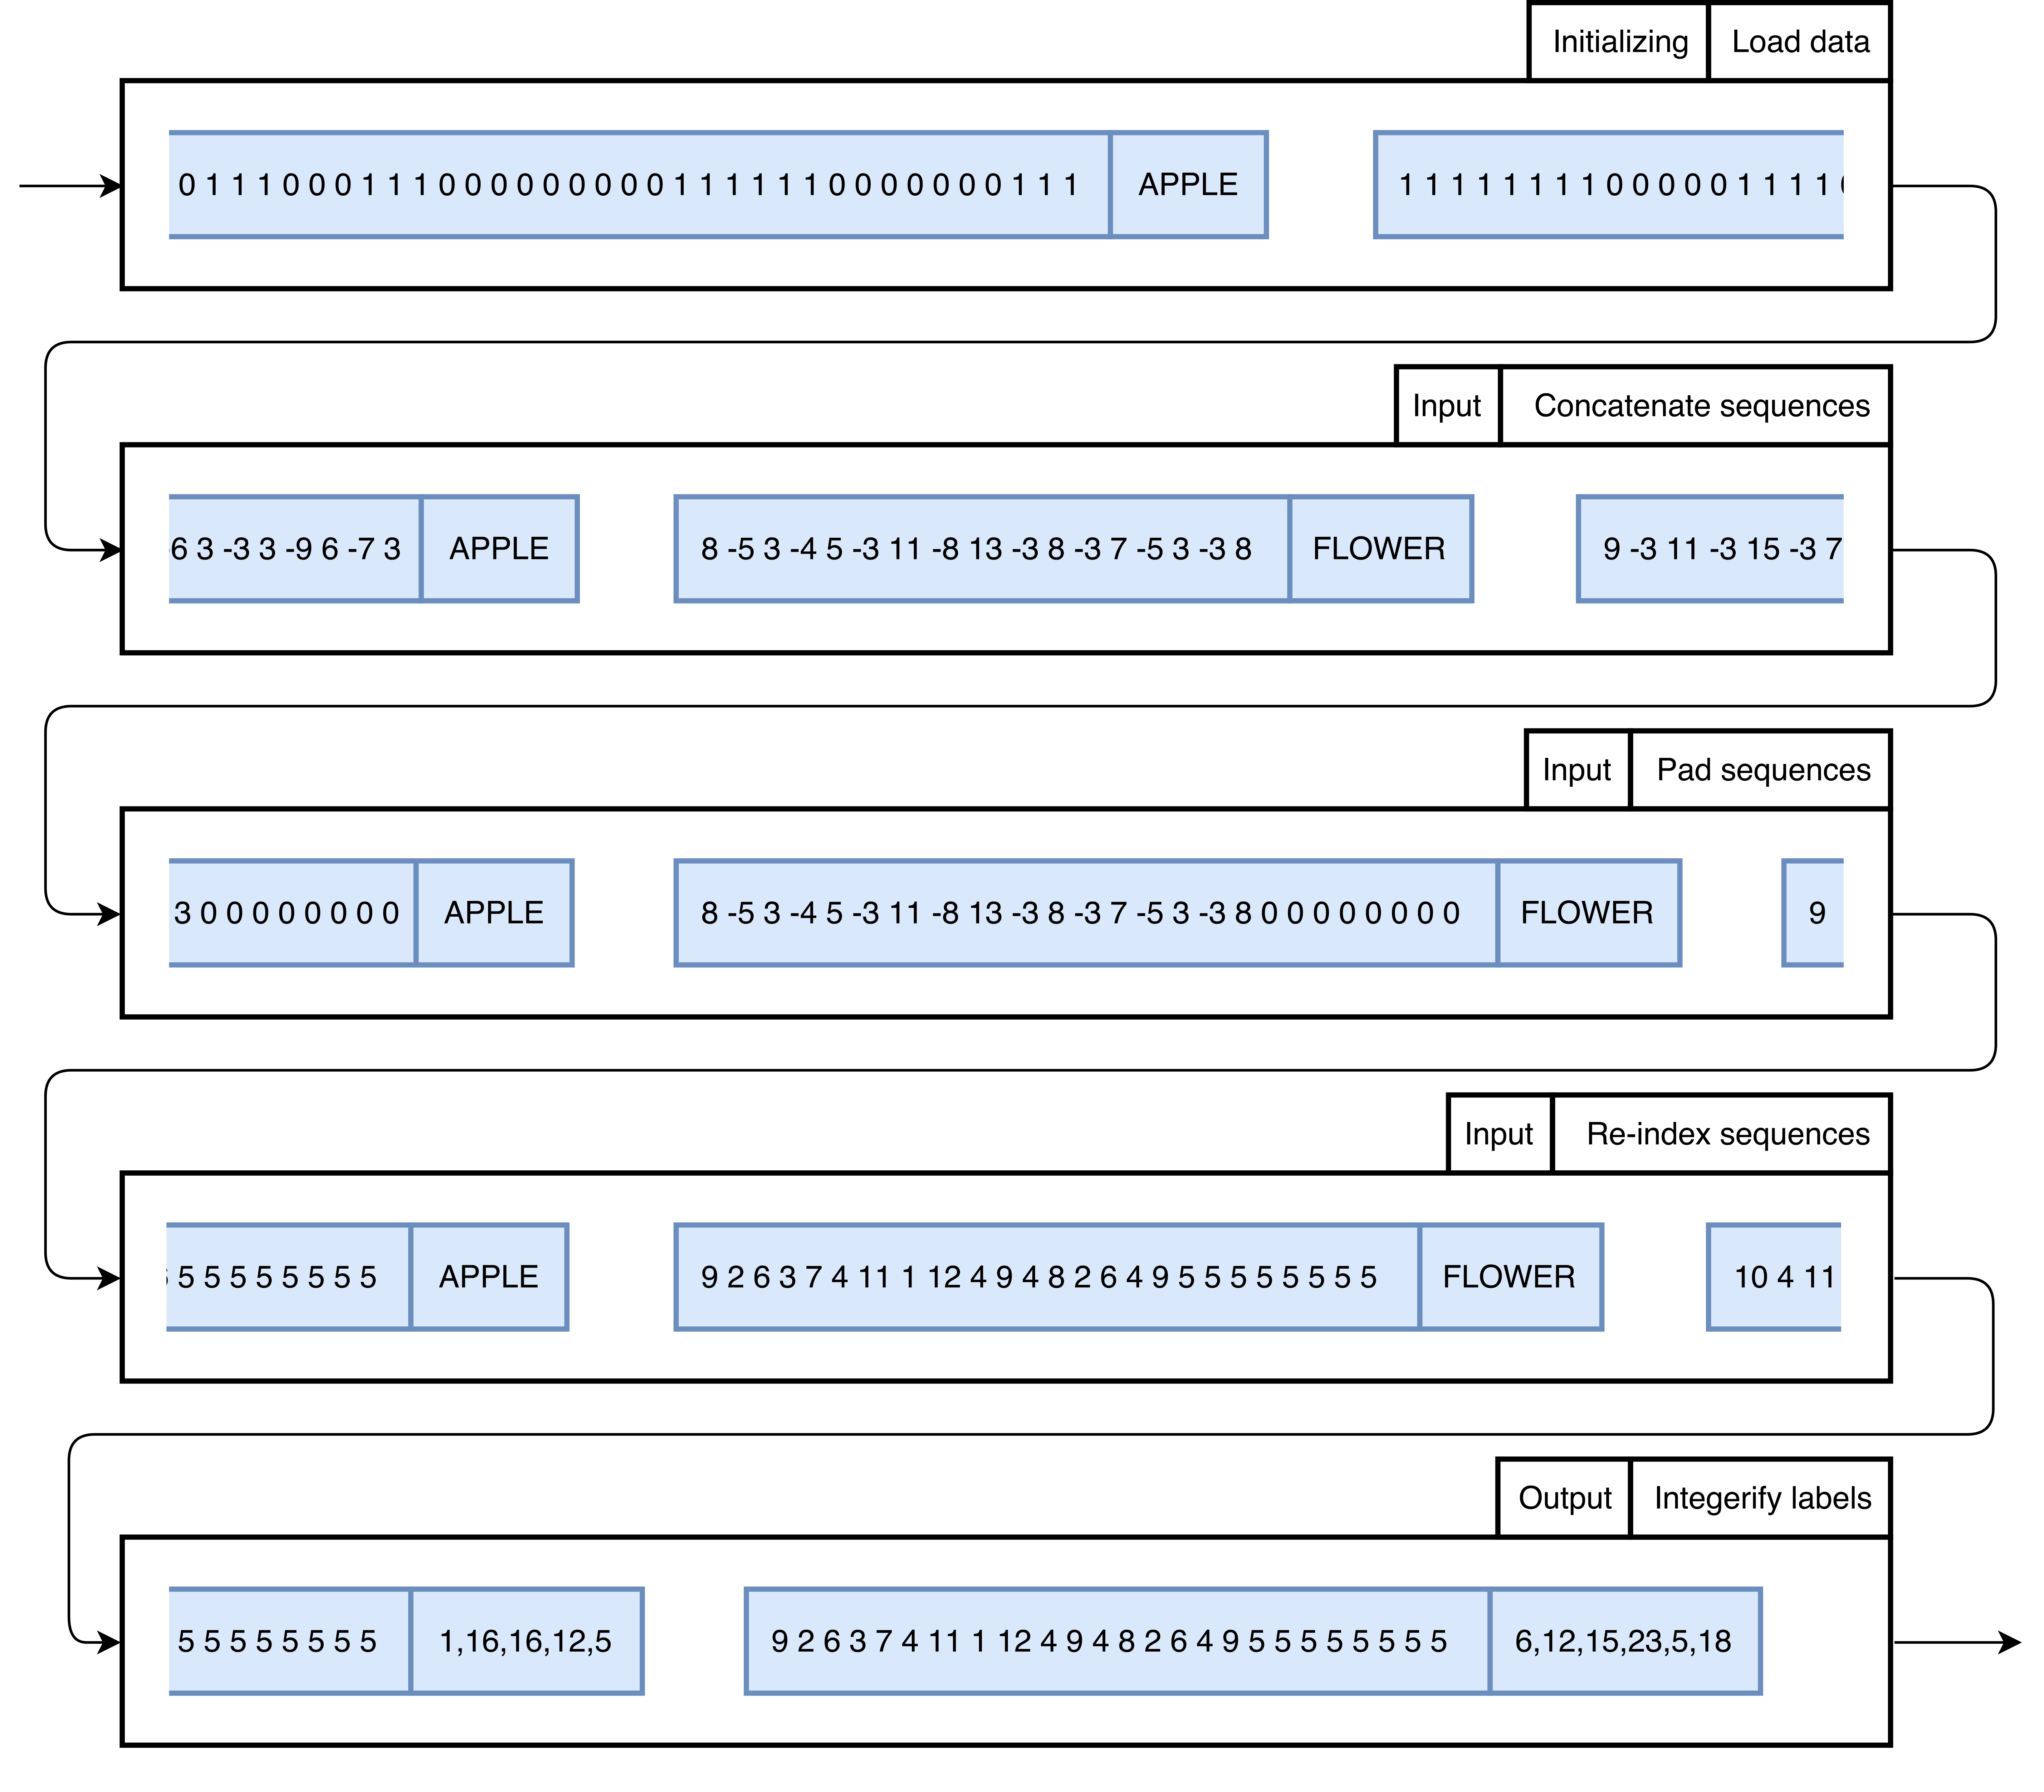
\includegraphics[width=1\textwidth]{fig/development_process/transformator.png}
    \caption{Illustration of handlers transforming data}
    \label{fig:development-transformator}
\end{figure}

Figure \ref{fig:development-transformator} illustrates a sequence of handlers, each transforming the data in one specific way. The first handler initiates the data by loading the binary data from the {\tt Preprocessor}. The second handler concatenates the binary data into sequences, where positive integers indicate a series of white pixels, and a negative integer indicates a series of black pixels. The third handler applies padding, to ensure that all the data has the same width before feeding it to the models. The padding is done by appending zeros at the end of the original sequence. The second last handler re-indexes the data, as our models expect unsigned integer values. The final handler transforms the labels from letters to an integer value, here we have given each letter the value that corresponds to their number in the English alphabet.

\subsection{Noise}
A special handler was implemented to add noise to the data. This handler iterates over the binary bits from the raw pixel data, and with a given probability sets a random bit value \(1\) or \(0\). The handler accepts a threshold in percent, which governed how often the bits can be randomized. Because the handler does not take into account the original value of the bit, the handler with a threshold \(T\) will on average change a big-value with probability approximately \(\frac{T}{2}\).